\documentclass{standalone}

\usepackage{tikz}
\usetikzlibrary{arrows}
\usetikzlibrary{decorations.markings}

\begin{document}

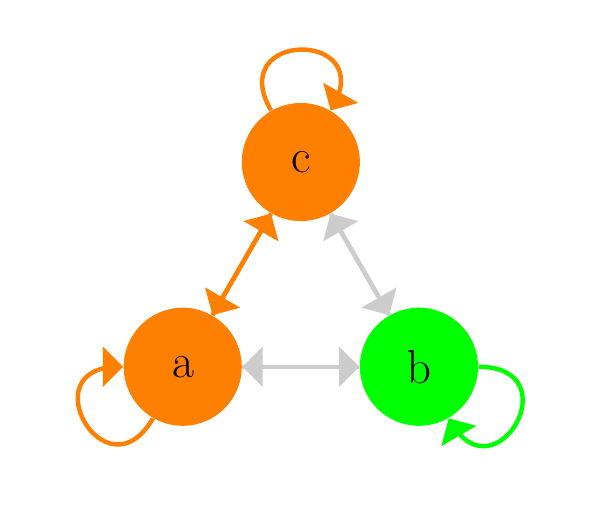
\begin{tikzpicture}
  \node (a) [style={minimum size=1.5cm,fill=orange,text=black,shape=circle}] at (0, 0) {\LARGE{a}};
  \node (b) [style={minimum size=1.5cm,fill=green,text=black,shape=circle}] at (3, 0) {\LARGE{b}};
  \node (c) [style={minimum size=1.5cm,fill=orange,text=black,shape=circle}] at (1.5, 2.6) {\LARGE{c}};

  \draw[draw=black!20!white, ultra thick, -triangle 90] (a) -- (b);
  \draw[draw=black!20!white, ultra thick, -triangle 90] (b) -- (a);

  \draw[draw=black!20!white, ultra thick, -triangle 90] (b) -- (c);
  \draw[draw=black!20!white, ultra thick, -triangle 90] (c) -- (b);

  \draw[draw=orange, ultra thick, -triangle 90] (a) -- (c);
  \draw[draw=orange, ultra thick, -triangle 90] (c) -- (a);

  \draw[draw=orange, ultra thick, -triangle 90] (a) to [out=-120,in=180,looseness=4] (a);

  \draw[draw=green, ultra thick, -triangle 90] (b) to [out=0,in=300,looseness=4] (b);

  \draw[draw=orange, ultra thick, -triangle 90] (c) to [out=-240,in=-300,looseness=4] (c);

\end{tikzpicture}

\end{document}
